\documentclass[10pt]{article}
\usepackage{geometry}
\geometry{a4paper} 
\usepackage{graphicx}
\usepackage{fancyhdr}
\usepackage{float}
\pagestyle{fancy}
\setlength\headheight{26pt}
\lhead{
\includegraphics[width=3cm]{edem_logo.jpg}}
\rhead{Computer Science Partial}
\usepackage{lipsum}
\usepackage{xcolor}

\usepackage{titlesec}
\usepackage[many]{tcolorbox}

% Adjust spacing after the chapter title
\titlespacing*{\chapter}{0cm}{-2.0cm}{0.50cm}
\titlespacing*{\section}{0cm}{0.50cm}{0.25cm}

% Indent 
\setlength{\parindent}{0pt}
\setlength{\parskip}{1ex}

% Sections in new page
\let\OldSection\section
\renewcommand{\section}{\clearpage\OldSection}

% --- Theorems, lemma, corollary, postulate, definition ---
% \numberwithin{equation}{section}

\newtcbtheorem[]{card}{Card}%
    {enhanced,
    colback = black!5, %white,
    colbacktitle = black!5,
    coltitle = black,
    boxrule = 0pt,
    frame hidden,
    borderline west = {0.5mm}{0.0mm}{black},
    fonttitle = \bfseries\sffamily,
    breakable,
    before skip = 3ex,
    after skip = 3ex
}{card}

\tcbuselibrary{skins, breakable}

% exam-cover.tex — reusable cover page for exams
% Usage:
%   \input{exam-cover}                       % in preamble or after \begin{document}
%   \examsetup{Course}{Program}{Year}{Type}{Date}{Duration}
%   \begin{document}
%   \makeexamcover
%   ... exam content ...

% Appearance variables for exam regulations
\providecommand{\ExamRegBgColor}{gray!12}   % background color
\providecommand{\ExamRegPadding}{8pt}       % inner padding of the box
\providecommand{\ExamRegFont}{\small}       % one-point smaller than the base class

% ---------- Variables (defaults) ----------
\providecommand{\ExamCourse}{Course Name}
\providecommand{\ExamProgram}{Program / Cohort}
\providecommand{\ExamYear}{2025--2026}
\providecommand{\ExamType}{Final Exam}
\providecommand{\ExamDate}{DD/MM/YYYY}
\providecommand{\ExamDuration}{2h 30m}

% Convenience setup: \examsetup{Course}{Program}{Year}{Type}{Date}{Duration}
\newcommand{\examsetup}[6]{%
  \renewcommand{\ExamCourse}{#1}%
  \renewcommand{\ExamProgram}{#2}%
  \renewcommand{\ExamYear}{#3}%
  \renewcommand{\ExamType}{#4}%
  \renewcommand{\ExamDate}{#5}%
  \renewcommand{\ExamDuration}{#6}%
}

% ---------- Regulations ----------
\newcommand{\ExamRegulations}{%
\usepackage{}
\begingroup
    \ExamRegFont
    \setlength{\fboxsep}{\ExamRegPadding}% padding inside the color box
    \colorbox{\ExamRegBgColor}{%
      \parbox{0.95\linewidth}{%
        \setlength{\parindent}{0pt}%
        % (Optional) tighten list spacing a touch:
        \setlength{\itemsep}{0.3em}%
        \setlength{\parsep}{0pt}%
        \setlength{\topsep}{0.3em}%
        \begin{enumerate}
            \item \textbf{You cannot be late.} The exam will start punctually which means that any student that arrives after the start time will not be permitted entry. Students who are late will not be allowed to participate in the examination session.
            \item Students are permitted to ask questions about the examination paper during the first \textbf{30-45 minutes}. To do this, students must raise their hands and wait for the professor's permission. Each question must be asked out loud so that all students have equal access to the information. It is strictly prohibited to ask questions beyond this designated time period.
            \item Any electronic device (mobile phone, iPad, smartwatch, computer etc.) \textbf{is not permitted in the examination room.} If a student is found in possession of any of these it will result in immediate \textbf{expulsion} from the exam room and the student's examination session will be graded as \textbf{"Fail"}.
            \item The student must not bring notes and materials of the subject (or any other) into the examination room. Students should make sure that \textbf{drawers} under the tables are empty. \textbf{Each student will be responsible for the area} in which they are located meaning that if notes or other prohibited material that does not belong to them are found in this area it will still be their responsibility.
            \item \textbf{Students must have all necessary material to complete the exam} as they are not permitted to request anything from their classmates (eg. calculator, pens, rulers etc.). They are not permitted to be in possession of anything that the professor has not authorized.
            \item \textbf{Communication between students during the examination session is strictly prohibited}. Students who attempt to communicate (for example through talking, the passing of notes, the exchange of papers or any other form including inappropriate behaviours) will be subject to \textbf{expulsion}. The exam will be automatically confiscated and the student's examination session will be graded as "Fail".
            \item \textbf{Once the examination session has begun, students are not permitted to leave the examination room under any circumstances before submitting their examination paper.} If a student does leave, then this will be interpreted as a withdrawal from the exam resulting in the examination session being graded as a "Fail".
            \item Once a student has left the examination room \textbf{they are prohibited reentry.}
            \item \textbf{Students must submit the exam within the stipulated period} meaning that they are not able to request extensions.
            \item Upon completion, \textbf{students must hand in their examination paper and sign a submission form before leaving the examination room.} They must do this in order for the exam paper to be successfully submitted.
\end{enumerate}
}% end parbox
    }% end colorbox
  \endgroup
}

% ---------- Cover builder ----------
\newcommand{\makeexamcover}{%
  \begin{coverpage}
    \thispagestyle{fancy}
    % Header
    \begin{center} 
        \vspace*{0.2cm}
        {\LARGE \textbf{\ExamCourse} -- \textbf{\ExamType} \par}
        {\large \ExamProgram\ \textbullet\ \ExamYear\par}
    \end{center}

    \vspace{0.2cm}
    % (Name + Group on ONE line using a single tabular
    \noindent
    \begin{tabular}{@{}p{0.65\linewidth} p{0.3\linewidth}@{}}
      \textbf{Name and Surname:} \hrulefill & \textbf{Group: } \hrulefill \\
    \end{tabular}
    \vspace{0.6em}

    % Date + Duration 
    \noindent
    \begin{tabular}{@{}ll@{}}
      \textbf{Date:} & \ExamDate \\[0.3em]
      \textbf{Duration:} & \ExamDuration \\
    \end{tabular}

    \vspace{0.6em}

    % Exam regulations
    {\large \textbf{Exam Regulations}}\par
      \ExamRegulations

    \vfill

  \end{coverpage}
  \clearpage
}  % load the cover macros

% Set variables (either here or just before \begin{document})
\examsetup{Computer Science}{IGE – 1st Year}{2025--2026 Edition}{Partial Exam}{13/11/2026}{1h 45m}


\begin{document}

%==========================
% Alternative Exam A
%==========================
\makeexamcover

\section*{Unit 1 Problems (2.0 points total)}

\subsection*{Q1 - CPU execution}
A processor has four registries, labeled R0, R1, R2, and R3 and the following set of operation codes: 
\begin{enumerate}
    \item \texttt{0001} Addition
    \item \texttt{0010} Substraction
    \item \texttt{1100} Multiplication
    \item \texttt{1101} Integer Division
    \item \texttt{1110} Modulo (reminder after Integer division)
\end{enumerate}
The 10-bit instruction is formatted as follows. 

\texttt{Opcode(4) | Dest(2) | Src1(2) | Src2(2)}

For example, the instruction \texttt{1110 00 01 10} means "calculate the reminder after Integer division of the value of registry R1 divided by the value of registry R2 (R1 modulo R2), and store the value in registry R0".

The initial value in the registers are in table \ref{tab:initial_state}: 

\begin{table}[H]
    \begin{tabular}{ll}
        R0 & \textt{0b1011}\\
        R1 & \textt{0b1000}\\
        R2 & \textt{0b0010}\\
        R3 & \textt{0b0000} \\ 
    \end{tabular}
    \caption{Initial states}
    \label{tab:initial_state}
\end{table}



Answer the following questions: 
\begin{enumerate}
    \item Convert to decimal the values in registry (prefixed with \verb|0b|). \textbf{(0.5 pts)}
    
    \textbf{Solution:}
    \begin{itemize}
        \item R0 = 0b1011 = 11
        \item R1 = 0b1000 = 8
        \item R2 = 0b0010 = 2
        \item R3 = 0b0000 = 0
    \end{itemize}
    \item Write the instruction to add the values in registries R1 and R2 and store it back in registry R2. This instruction will be instruction 1. \textbf{(0.2 pts)}\\
    
    \textbf{Solution:}
    
    Opcode for ADD = \texttt{0001}\\
    Dest = R2 = \texttt{10}\\
    Src1 = R1 = \texttt{01}\\
    Src2 = R2 = \texttt{10}\\
    
    Final instruction:
    \[
    \texttt{0001\,10\,01\,10}
    \]

    \item Consider the following instructions:
    \begin{itemize}
        \item Instruction 2: 0010000001
        \item Instruction 3: 1110110100
    \end{itemize}
    Explain what every instruction will do.(0.3 pts)

    \textbf{Solution:}
    \begin{itemize}
        \item Instruction 2: \texttt{0010 00 00 01}  
        Opcode 0010 = subtraction.  
        R0 = R0 - R1.
        
        \item Instruction 3: \texttt{1110 11 01 00}  
        Opcode 1110 = modulo.  
        R3 = R1 mod R0.
    \end{itemize}
    \textbf{(0.3 pts)}
    \item Using the initial state, apply instruction1, instruction2 and instruction3. Show the state
of the registers after the execution of every instruction. \textbf{(1 pts)}      

\textbf{Solution:}
\begin{enumerate}
\item \textbf{Instruction 1: ADD R1 and R2 → R2}  

R2 = 8 + 2 = 10  
R2 = \texttt{0b1010}

Registers:  
\[
\begin{aligned}
R0 &= 11\;(\texttt{0b1011})\\
R1 &= 8\;(\texttt{0b1000})\\
R2 &= 10\;(\texttt{0b1010})\\
R3 &= 0\;(\texttt{0b0000})
\end{aligned}
\]

\item \textbf{Instruction 2: SUB R0 = R0 - R1}  

R0 = 11 - 8 = 3  
R0 = \texttt{0b0011}

Registers:  
\[
\begin{aligned}
R0 &= 3\;(\texttt{0b0011})\\
R1 &= 8\;(\texttt{0b1000})\\
R2 &= 10\;(\texttt{0b1010})\\
R3 &= 0\;(\texttt{0b0000})
\end{aligned}
\]

\item \textbf{Instruction 3: MOD R3 = R1 mod R0}  

R3 = 8 mod 3 = 2  
R3 = \texttt{0b0010}

Final registers:  
\[
\begin{aligned}
R0 &= 3\;(\texttt{0b0011})\\
R1 &= 8\;(\texttt{0b1000})\\
R2 &= 10\;(\texttt{0b1010})\\
R3 &= 2\;(\texttt{0b0010})
\end{aligned}
\]
\end{enumerate}

\end{enumerate}


\section*{Unit 2 --- Problems (3 points total)}
\subsection*{Code Card 1 — Find the bug (0.75 pt)}
The intended behavior of Card 1 is to print "ok" when the variable \verb|code| is equal to the literal string \verb|"OK"|. Underline the incorrect line and write the minimal correction. Motivate your response.

\begin{card}{ Card 1}{card-1}
\begin{verbatim}
code = OK
if code is OK:
    print("ok")
\end{verbatim}
\end{card}

\subsubsection*{Solution}
The minimal change is to add double quotations to the literal \verb|"OK"| and replace \verb|code is OK| with \verb|code == "OK"|,  as it is the correct syntax to make an exact comparison. The operator \verb|is| is not for comparing values but is actually used to test object identity (if two variables point to the same object in memory). 

\subsubsection*{Rubric}
0.6 for the change code and 0.15 for the explanation. 

\subsection*{Code Card 2 -- Predict the result (0.75 pt)}
 Trace the execution of the while loop and predict exactly what is printed. Briefly explain your result

\begin{card}{ Card 2}{card-2}
\begin{verbatim}
i = 0
while i < 5:
    i += 1
    if i % 2 == 0:
        continue
    print(i, end="")
\end{verbatim}
\end{card}

\subsubsection*{Solution} 
The loop prints \verb|135|. The first if clause uses \verb|continue| to skip event numbers, and the keyed argument \verb|end=""| replaces the default new line introduced after each call to the function \verb|print| by an empty character. 

\subsubsection*{Rubric}
0.5 points for the integer number sequence. 0.15 points for keyed argument. 0.1 for explanation.

\subsection*{Code Card 3 -- Bug fix and explain (0.75 pt)}
Fix the code below to achieve the stated intent: sum of squares of numbers divisible by 3 from \verb|a| to \verb|b|, both included.

\begin{card}{ Card 3 }{card-3}
\begin{verbatim}
a = 1
b = 10
total = 0
for n in range(a, b):       
    if n % 3:               
        total += n*n
print(total)
\end{verbatim}
\end{card}

\subsubsection{Solution}
The error is in the call `range(a,b)` which is not inclusive, as it will not include \verb|b|. It should be replaced by `range(a,b+1)`.

\subsubsection{Rubric}
0.65 for fixing the error and 0.1 for the explanation. 

\subsection*{Code Card 4 -- Bug fix (possibly) and explain (0.75)}
Review the function \verb|head| below to achieve the following behavior: Return the \verb|n| first elements of a list \verb|l| passed as argument, optionally with step \verb|s| (default step should be 1). Identify and correct potential failures. Briefly motivate your response.

\begin{card}{ Card 4}{card-4}
\begin{verbatim}
def head(l, n, s):
    return s[:-n]    
my_list = [1, 2, 3, 4, 5]
print(head(my_list, 2)) # Expected [1, 2] 
\end{verbatim}
\end{card}

\subsubsection*{Solution}
The function does not have any default step, which should be 1. The parameters \verb|l|, and \verb|s| are not used correctly either. It does not use the parameter \verb|l| as a list or \verb|s| to slice, so, instead, it should be written as: 
\begin{card} { Card 4 Solution}{card-5}
\begin{verbatim}
def head(l, n, s=1):
    return l[:n:s]    
my_list = [1, 2, 3, 4, 5]
print(head(my_list, 2)) # Expected [1, 2]  
\end{verbatim}
\end{card}

\subsubsection*{Rubric}
0.5 points for fixing the use of parameters in the return statement, and 0.25 for fixing the function signature.

\section*{Unit 3 Problems (5 points total)}

\subsection*{Q1 — Error Detection \& Correction (1.5)}
Consider the following code, it contains several syntax/logic errors.
\begin{verbatim}
const int led1 = 11
const int led2 = 2;
const int btn = 11;

void setup() {
    pinMode(led1, OUTPUT)
    pinMode(led2, OUTPUT);
    pinMode(btn, OUTPUT);
}

void setup() {
if (digitalRead(btn) = HIGH) {
    pattern = !pattern;
    }
    if (pattern = true) {
        digitalWrite(led1, HIGH);
        digitalWrite(led2, LOW);
    } else {
        digitalWrite(led1, HIGH);
        digitalWrite(led2, HIGH)
        delay(300);
        digitalWrite(led1, LOW);
        digitalWrite(led2, LOW);
    }
    delay(300)
}
\end{verbatim}

Solve the following items:
\begin{enumerate}
    \item Find all 9 errors in the code (0.5 pts).

    \textbf{Solution:}
    There's actually 10 errors in the code, finding 9 gets you all the points:
    \begin{enumerate}
        \item Missing semicolon: \verb|const int led1 = 11;|
        \item Wrong button pin (same as LED1): should not be 11.  
        Fix: \verb|const int btn = 3;| (or another free pin).
        \item \verb|pinMode(led1, OUTPUT)| missing semicolon.
        \item \verb|pinMode(btn, OUTPUT);| must be \verb|INPUT|.
        \item Second function named \texttt{setup()}. Must be \texttt{loop()}.
        \item Assignment used instead of comparison: \verb|digitalRead(btn) = HIGH| → \verb|==|.
        \item Variable \texttt{pattern} not declared. Must declare: \verb|bool pattern = false;|.
        \item Condition \verb|if (pattern = true)| uses assignment. Should be \verb|if (pattern == true)| or simply \verb|if(pattern)|.
        \item Missing semicolon in \verb|digitalWrite(led2, HIGH)|.
        \item Missing semicolon in \verb|delay(300)|
    \end{enumerate}

    \item For every error, explain why it’s an error and how to fix it (0.5 pts).

    \textbf{Solution:}
    \begin{itemize}
        \item \textbf{Missing semicolons:} C++ uses semicolon to signal when one instruction finishes and the following starts so it's mandatory to add them at the end of every instruction
        \item \textbf{== instead of =:} In C++ and many other languages, using = will mean assign a value to a variable, in these cases we don't want to change the value of the variable but to check if it has a certain value, therefore we must use double equal.
        \item \textbf{Wrong button pin:} you can't connect 2 devices to the same Arduino Pin
        \item \textbf{INPUT/OUTPUT:} A button is an element from which we are going to read a value, not to write any value in it, therefore we must use INPUT, not OUTPUT whe we set the pin mode.
        \item \textbf{variable pattern}: In order to use a variable, first we have to save space in the computer's memory, doing this is called declaring the variable.
    \end{itemize}
    
    \item Explain what the corrected code is doing (0.5 pts).

    \textbf{Solution:}
    The code reads a pushbutton. When the button is pressed, the Boolean variable \texttt{pattern} toggles.  
    When \texttt{pattern} is true, the LEDs stay in a fixed on/off pattern, when \texttt{pattern} is false, they blink together every 300 ms.

\end{enumerate}

\subsection*{Q2 - Referee table (1.5)}
The following schematic represents your prototype board. The integrated protoboard includes 2 push buttons, labeled as B1, and B2, and two (pull-down resistors). The objective of the prototype is to provide an electronic table to keep track of the score in a football match. Push-button B1 is used to control the score of the local team  and B2 is used to control the score of the visiting team (1 push increases the score in 1). 
\begin{figure} [H]
    \centering
    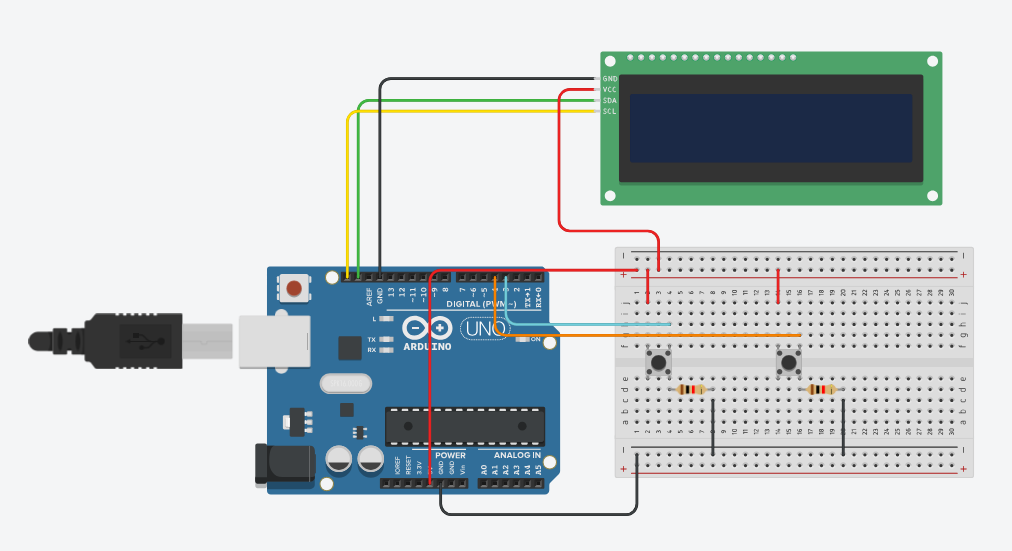
\includegraphics[width=1\linewidth]{CircuitSolved.png}
    \caption{EDEM League electronic table}
    \label{fig:placeholder}
\end{figure}

Based on the provided information and diagram, follow the instructions below to complete the
wiring of the prototype.
\begin{enumerate}
    \item Draw over the diagram the wires needed to connect the circuit (0.5 pts)
    \begin{enumerate}
        \item Complete the variables, constants needed. (0.5 pts)

        \textbf{Solution:}
        We need to add constants for the pins that connect the buttons, and variables to keep track of the amount of points that each team has.
        \begin{verbatim}
            #include <Adafruit_LiquidCrystal.h>
            
            Adafruit_LiquidCrystal lcd(0);
            
            const int B1 = 2;
            const int B2 = 3;
            
            int scoreLocal = 0;
            int scoreVisitor = 0;
        \end{verbatim}
        \item Complete the setup function (1 pts)
        \textbf{Solution:}

        \begin{verbatim}
        void setup() {
          lcd.begin(16, 2);
        
          pinMode(B1, INPUT);
          pinMode(B2, INPUT);
        
          lcd.print("EDEM league");
        }
        \end{verbatim}
    
        \item Complete the loop function (1.5 pts)

        \textbf{Solution:}

        \begin{verbatim}
            void loop() {
              bool b1 = digitalRead(B1);
              bool b2 = digitalRead(B2);
            
              if (b1 == HIGH) {
                scoreLocal += 1;
              }
              if (b2 == HIGH) {
                scoreVisitor += 1;
              }
            
              lcd.setCursor(0, 1);
              lcd.print(scoreLocal);
              lcd.print(" - "); // clear residual digits
              lcd.print(scoreVisitor);
            
              delay(100);
            }
        \end{verbatim}

    \end{enumerate}
\end{enumerate}

To write the code, you can base it on this example of how an LCD screen works, provided as an
example in the next page.

\subsection{Example code}
This code will turn on the LCD screen, write ”hello world” in the first line, and then, in the
second line, it writes, every second, the amount of seconds that it has been working. You can
use this code as inspiration to write the code of the last exercise.

\begin{verbatim}
#include <Adafruit_LiquidCrystal.h>
int seconds = 0;
Adafruit_LiquidCrystal lcd_1(0);
void setup()
{
    lcd_1.begin(16, 2);
    lcd_1.print("hello world");
}
void loop()
{
    lcd_1.setCursor(0, 1);
    lcd_1.print(seconds);
    delay(1000); // Wait for 1000 milliseconds
    seconds += 1;
}    
\end{verbatim}
\end{document}
